% Chapter 3

\chapter{Literature Review} % Main chapter title

\label{review} % For referencing the chapter elsewhere, use \ref{Chapter1} 

\lhead{Chapter 3. \emph{Literature Review}} % This is for the header on each page - perhaps a shortened title
\doublespacing
\setlength{\parindent}{1cm}
\section{Identifying High Quality Informative Content in Social Media}
Identifying high quality content from the social media feeds that are related to events, is one of the main objectives of our research. As already discussed in Chapter \ref{events}, presence of spams, phishing, farm links, promotion of irrelevant content and development of nepotistic relationships are some of the major concerns of information quality in social media. Several effective solutions has been proposed in combating them by \cite{benevenuto2010detecting,chhabra2011phi,grier2010spam,yardi2009detecting}. Among the different facets of information quality, credibility and trustworthiness of the references are also important.  Due to the popularity and its ability to broadcast information at a tremendous pace, social media is also sometimes used by malicious users to spread misinformation and rumors \cite{tonkin2012twitter}. In such cases, it becomes necessary to assess the credibility and trustworthiness of the information posted. It was showed by Castillo et al. \cite{castillo2011information} that selection of different types of features and automated classification based on supervised training can be used for detecting credible information about newsworthy topics in Twitter. In one of their works \cite{agichtein2008finding} they also proposed a general classification framework for identifying high quality social media content. They took into account the rich meta data like links between items and explicit quality ratings available in Yahoo! Answers website to train a supervised classification model. Credibility of events in Twitter was studied by Gupta et al. \cite{gupta2012evaluating}. They used PageRank for propagating credibility scores on a heterogeneous network of events, tweets and users. They further constructed a graph between similar events and propagated the scores of the events from the previous network to estimate the credibility of other events. Ranking of tweets based on their credibility during trending events was proposed by Gupta and Kumaraguru \cite{gupta2012credibility}. They showed automated extraction of credible information from Twitter, by adopting supervised learning combined with relevance feedback approach using different features mined from tweets and the users posting them. Truthy\footnote{http://truthy.indiana.edu/}, was developed by Ratkiewicz et al. to study information diffusion on Twitter and compute a trustworthiness score for a public stream of micro-blogging updates related to an event to detect political smears, astroturfing, misinformation, and other forms of social pollution \cite{ratkiewicz2011truthy}.


Several mechanisms for ranking social media content in terms of their informativeness have been proposed. Ranking of microblogs like tweets are of particular interest to us as we consider tweets as a representative of short textual content produced in social media. There are many web hosted applications that supplements the default search provided by Twitter in order to effectively retrieve relevant and high quality tweets from different perspectives\footnote{\tiny http://mashable.com/2009/04/22/twitter-search-services}. On going through these services we found that the most commonly used criteria for ranking tweets are recency, popularity based on retweets and favorite counts, authority of the users posting the tweets and content relevance. Twitter itself uses the popularity of the tweets and features mined from the profile of the users in order to provide personalized search results ordered by recency\footnote{\tiny https://blog.twitter.com/2011/engineering-behind-twitter\%E2\%80\%99s-new-search-experience}. A study of different state-of-the-art features and approaches commonly used for ranking tweets has been documented by \cite{Damak2013, nagmoti2010ranking}. Seen\footnote{\tiny http://seen.co} is a new state-of-the-art platform that uses a proprietary algorithm named \textit{SeenRank} for ranking event related tweet content for presenting event highlights and summaries. In this work, we consider \textit{SeenRank} as one of our baselines. As the number of retweets of a tweet is widely used for ranking, we also use it as one of our baselines. In the context of our work we name the ranking scheme as \textit{RTRank}

Apart from the existing real-world search applications, several adaptations of \textit{PageRank} \cite{page1999pagerank} has been proposed by the scientific community for ranking tweets and users in Twitter \cite{weng2010twitterrank,tunkelang2009twitter, hallberg2012adaptation}. TweetRank \cite{hallberg2012adaptation} is one such adaptation that ranks tweets by taking into account the direct relationships between tweets in the form of retweets and replies, as well as indirect follower-friend relationships, and usage of similar hashtags. Various learning to rank approaches have been used for ordering tweets retrieved for a given query in terms of their relevance and quality \cite{Duan2010,mccreadie2013relevance,vosecky2012searching}. None of these ranking techniques have been devised for event-specific content. An attempt to solve a similar problem presented in this paper was made by \cite{becker2011selecting}. They represented tweets of an event in a cluster and calculated the similarity of individual tweets with the centroid of the cluster. Then they ranked the tweets based on the decreasing value of their similarity. We use this approach as one of our baselines.

Recently researchers have shown interest in investigating microblog summarization. Experiments have been conducted using both feature-based and graph-based approaches. However, in the context of our work only graph-based approaches are relevant. A comparison of different Twitter summarization algorithms was performed by \cite{inouye2011comparing}. Summarization of tweets for sporting events was performed by \cite{nichols2012summarizing} using the phrase graph algorithm \cite{sharifi2010experiments}. The popularly used graph-based summarization algorithms are \textit{LexRank} \cite{erkan2004lexrank} and \textit{TextRank} \cite{mihalcea2004textrank}. Both the algorithms make use of the PageRank scheme of ranking homogeneous nodes in a graph constructed from the text that needs to be summarized and identify the salient text units for producing the summary. Our algorithm uses a similar technique for heterogeneous nodes. Our proposed framework also defines the semantics of the relationships between the nodes differently in the context of tweets. We use both \textit{LexRank} and \textit{TextRank} as evaluation baselines.

%Although, we use some of the features used in the works related to ranking tweets and identifying credible content, our approach is entirely different from them. Moreover, we consider only those features that are intrinsic to tweet content. The presented model in this paper is an extension of \textit{Mutually Reinforcing Chain} framework \cite{wei2008}, to the Twitter environment, making our work more related to the graph-based summarization approaches. 

We propose implicit mutually reinforcing relationships between tweets, hashtags, text units, users and URLs forming a heterogeneous graph structure (\textit{TwitterEventInfoGraph}), which is novel and makes our work different from any prior work (refer Chapter \ref{eiim}). Scores are assigned to the association between the nodes representing the semantics of their relationships. We implement an iterative algorithm (\textit{TwitterEventInfoRank}) for ranking the nodes of the graph and propagating the event-specific scores of the nodes to its neighboring nodes based on the measure of their association. To our knowledge, this is the first work that identifies novel relationships between different units of content in Twitter and implements a graph-based algorithm for ranking them simultaneously in the context of an event.

\section{Entity Resolution}

Entity resolution has been known for more than five decades as the record linkage or the record matching problem in the statistics community \cite{fellegi1969theory,newcombe1959automatic,herzog2007data}. In the database community, the problem is defined as merge-purge \cite{hernandez1998real}, data de-duplication \cite{sarawagi2002interactive,ananthakrishna2002eliminating}, and instance identification \cite{wang1989inter}. In the Artificial intelligence community, this problem is described as database hardening \cite{cohen2000hardening}, and name matching \cite{bilenko2003adaptive}. The names co-reference resolution, identity uncertainty, and duplicate detection are also commonly used to refer to the same task \cite{elmagarmid2007duplicate}. The term Entity Resolution (ER) first appeared in publications by researchers at the Stanford InfoLab led by Hector Garcia-Molina and is defined as the process of identifying and merging records judged to represent the same real-world entity \cite{garcia2006pair}. In the context of the work presented in this thesis a pre-defined real-life event is considered as an entity. For detailed definition of an event please refer Chapter \ref{events}.

Despite the differences in nomenclature used by these authors, the ER process actually comprises five major sub-tasks or activities \cite{talburt2011entity} which are
\begin{enumerate} 
\item	\textit{Entity reference extraction} – locating entity references in unstructured textual information.
\item	\textit{Entity reference preparation} – profiling, standardizing, cleaning, and enhancing reference information in preparation for resolution.
\item	\textit{Entity reference resolution} – the process or algorithm for determining when references are equivalent, often through direct matching of attributes.
\item	\textit{Entity identity management} - creating and maintaining persistent data structures that represent the identities of external entities, the focus of the proposed research.
\item	\textit{Entity relationship analysis} – exploring relationships among distinct entities such as household relationships or shared communication.
\end{enumerate}

The \textit{Event Identity Information Management} Life Cycle (Chapter \ref{eiim}) as proposed in this thesis reflects and implements all of the above activities. Historically the focus of ER research has been on Activity 3, the methods for carrying out the resolution process itself. The majority of published research literature falls into this area. The first formal model for resolution was the Fellegi-Sunter Model of Record Linkage \cite{fellegi1969theory}, which uses a decision-theoretic approach establishing the validity of principles first used in practice by Newcombe \cite{newcombe1959automatic}.  This was followed by the Stanford Entity Resolution Framework (SERF) developed at the Stanford InfoLab \cite{benjelloun2006generic}.  The SERF Model formalizes the generic ER problem as the interaction of two functions for comparing and merging records as black-boxes and defines the conditions required for these functions to give a unique ER result. It also formulates a family of so called ``Swoosh" algorithms (G-Swoosh, R-Swoosh, and F-Swoosh) for carrying out the ER process. With the rise of big data a distributed algorithm D-Swoosh \cite{benjelloun2007d}, was also proposed that can be implemented in a big data environment. More recently the Talburt-Wang Algebraic Model of ER has been proposed \cite{talburt2007algebraic} that views ER as a problem of partitioning a given set of references. 
 
In addition to research on Activity 3, there has also been extensive research in the area of information extraction (IE) that is directly related to the ER Activity 1, reference extraction. The task of entity extraction is also more relevant to social media, due to the unstructured nature of the content. One of the main emphases in the realm of unstructured textual content for last two decades has been in the task of extracting named entities and categorizing them into types. Competitions like MUC (Message Understanding Conference), CoNLL (Conference on Computational Natural Language Learning) and ACE (Automatic Content Extraction) spearheaded the development of new techniques in this domain. This led to the development of sophisticated tools like Stanford NER \cite{finkel2007named}, OpenNLP \cite{baldridge2005opennlp}, GATE \cite{cunningham2002gate}, LingPipe \cite{baldwin2003lingpipe} and NLTK \cite{bird2006nltk}. Variety of techniques ranging from hand-coded rules, automatic rules, to statistical machine learning techniques like hidden Markov models, maximum entropy and conditional random fields have been proposed. A comprehensive survey of the techniques could be found in \cite{piskorski2013information,sarawagi2008information}. A study of various efforts in extracting information from micro-blogs could be found in \cite{hua2012information} and a survey of named entity recognition and classification could be found in \cite{nadeau2007survey}. Efforts have been made by the industry in building crowd sourced knowledge bases like freebase \cite{bollacker2008freebase} and dbpedia \cite{auer2007dbpedia} for the purpose of entity extraction. A recent effort from the industry for extracting entities from social media and building scalable knowledge bases for doing so has been documented in \cite{deshpande2013building,gattani2013entity}. The rise of online social networks, has also motivated new research into the ER Activity 5, entity relationship analysis \cite{bilgic2006d}. With the rise of big data, the modern trend is to perform entity resolution process in humongous volumes of data and scale it horizontally \cite{kolb2012dedoop,talburt2015entity}. In spite of the recent efforts in the field of entity extraction and resolution from unstructured text, there is no generic framework that solves the problem of persistently collecting and managing entity identity information from social media. The development of Event Identity Information Management from social media is a pioneering effort in the field of entity resolution and would create new avenues of research.

Traditionally, entity identity resolution and management (Activity 4) has been a subject of system administration and management of user identities in large organizations. For the first time \cite{zhou2011entity}, showed the intersection of identity management, master data management and entity resolution could be used for managing identities of real-life entities in information systems, that could further play an important role in data integration and information quality. Entity identity management in social media mainly comprises of resolving and integrating profiles of the same person in social networking websites. The FOAF project has been playing an important role in all such efforts \cite{bouquet2010entity,bortoli2007foaf,raad2010user}. A very nice endeavor has been made by the OKKAM project for integrating and managing the multiple entity identifiers in various knowledge bases across the Internet \cite{bouquet2006okkam}. To our knowledge, we are the first to propose a framework for collecting and extracting identity information of events from social media and use the concepts of entity identity management and entity resolution for persistently managing their identities with respect to time.


\section{Event Identification in News Text}
The event detection task \cite{allan2002topic} in the TDT program (Topic Detection and Tracking), led to significant advancements in the field of event-based organization of broadcast news. Some of the efforts in the TDT program focused on online event detection from continuous and real-time streams of textual news documents in newswires \cite{allan1998line,kumaran2004text}. While others explored the detection of past events from archived news documents \cite{yang1998study}. 

The textual content in news documents are different from the short informal text common in the realm of social media.  Most of these documents contain formal text with well-formed grammatical structures, enabling the researchers to rely on the state-of-the-art natural language processing techniques. Named entity extraction and Parts-of-Speech (POS) tagging are among the widely used techniques. Zhang et al. \cite{zhang2007new} extracted named entities and POS tags from textual news documents, and used them to reweigh tf-idf representations of these documents for the new event detection task. Filatova and Hatzivassiloglou \cite{hatzivassiloglou2003domain} identified named entities corresponding to participants, locations, and times in text documents, and then used the relationships between certain types of entity pairs to detect event content. Hatzivassiloglou et al. \cite{hatzivassiloglou2000investigation} used linguistic features (e.g., noun phrase heads, proper names) and learned a logistic regression model for combining these features into a single similarity value. Makkonen et al. \cite{makkonen2004simple} extracted meaningful semantic features such as names, time references, and locations, and learned a similarity function that combines these metrics into a single clustering solution. 

Extracting events from text has been the focus of numerous studies as part of the NIST initiative for Automatic Content Extraction (ACE) \cite{ahn2006stages,ji2008refining}. The ACE program defines event extraction as a supervised task, given a small set of predefined event categories and entities, with the goal of extracting a unified representation of the event from text
via attributes (e.g., type, subtype, modality, polarity) and event roles (e.g., person, place, buyer, seller). Ahn \cite{ahn2006stages} divided the event extraction task into different subtasks, including identification of event keyword triggers, and determination of event
coreference, and then used machine learning methods to optimize and evaluate the results of each subtask. Ji and Grishman \cite{ji2008refining} proposed techniques for extracting event content from multiple topically similar documents, instead of the traditional approach of extracting events from individual documents in isolation. In contrast with the predefined templates outlined by ACE, Filatova et al. \cite{filatova2006automatic} presented techniques to automatically create templates for event types, referred to as domains, given a set of domain instances (i.e., documents containing information related to events that belong to the domain). 

As already discussed, social media documents are extremely concise, noisy and lacks well-established grammatical structures. Therefore, the techniques used in these works are not always suitable for identification of events from social media.  It has been shown that it is extremely challenging for the state-of-the art information extraction algorithms to perform efficiently and give accurate results for micro-blogs \cite{derczynski2013microblog}. For example, named entity recognition methods typically show 85-90\% accuracy on longer texts, but 30-50\% on tweets \cite{ritter2011named}. Therefore, new approaches had to be taken, leading to new techniques for detecting events in social media, which we discuss next.

%One of the goals of the EIIM framework presented in this thesis, is to identify and track event related content being generated in social media. However, the framework does not require detection of unknown events from real-time streams of social media messages. Instead it is provided with a predefined set of events along with predefined hashtags for the respective events, which are used for relevant data collection.

\section{Event Identification in Social Media}
Identification of events and event related content from social media is still in its infancy and needs to be studied more. Several related papers explored the unknown event identification scenario in social media.
Weng and Lee \cite{weng2011event} proposed wavelet-based signal detection techniques for identifying
real-life events from Twitter. These techniques can detect significant bursts or trends
in a Twitter data stream. Sankaranarayanan et al. \cite{sankaranarayanan2009twitterstand}
identified late breaking news events on Twitter using clustering, along with a text-based
classifier and a set of handpicked news seeders. But they do not take into account the filtering of non-event content, which results in poor performance. Segregating the messages that have high likelihood of containing event related informative content from the ones with chances of having non-informative content, or content that are not at all related to an event are at the core of the work presented in this thesis.  Petrovic et al. \cite{petrovic2010streaming} used locality-sensitive hashing to detect the first tweet associated with an event in a stream of Twitter messages. Rattenbury et al. \cite{rattenbury2007towards} analyzed the temporal usage distribution of tags to identify tags that correspond to events. Chen and Roy \cite{chen2009event} used the time and location associated with Flickr image
tags to discover event-related tags with significant distribution patterns (e.g.bursts) in both of these dimensions. Becker et al. \cite{becker2010learning} defined multi-feature similarity metrics based on the textual and non-textual features associated with the social media documents in order to automatically identify events and their related content.
They use the general text-based classifier suggested in \cite{sankaranarayanan2009twitterstand} and a method for identifying top events suggested by \cite{petrovic2010streaming} as baseline approaches in their evaluations and achieved better precision scores.





% but, unlike our work in Chapter 4, they do not filter the vast
%amount of non-event content that exists on Twitter. This, unfortunately, results in poor
%performance, with very low precision scores compared with the precision achieved by our
%methods. Related to our work in Chapters 4 and 5, 



%As we discussed, such text-based and seeder-driven filtering of
%non-event data can be used to generate the event document stream we use in Chapter 5.

 
%
%%We use the general text-based classifier suggested in \cite{sankaranarayanan2009twitterstand} and a method for identifying top events suggested by Petrovic et
%%al. \cite{petrovic2010streaming} as baseline approaches in our evaluation of the unknown identification methods
%%of Chapter 4. While our work in the unknown event identification scenario focuses on timely, online, analysis, several efforts tried to address this task using retrospective analysis. 


New techniques have been proposed recently for identification of known events in social media.
Many of these techniques rely on a set of manually selected terms to retrieve event-related
documents from a single social media site \cite{sakaki2010earthquake,yardi2010tweeting}.  Sakaki et al. \cite{sakaki2010earthquake} developed
techniques for identifying earthquake events on Twitter by monitoring keyword triggers
(e.g., earthquake or shaking). In their setting, the type of event must be known a
priori, and should be easily represented using simple keyword queries. Benson et al. \cite{benson2011event} identified Twitter messages for concert events using statistical models to automatically tag artist and venue terms in Twitter messages.
Their approach is novel and fully automatic, but it limits the set of identified messages for
concert events to those with explicit artist and venue mentions. Most of these approaches are tailored towards one specific social media site. Becker et al. \cite{becker2012identifying} extracts event features, that are often noisy and missing and use them to develop query formulation strategies for retrieving content associated with a planned event from Twitter \cite{becker2011automatic} as well as different social media websites \cite{becker2012identifying}. 




Our method of tracking events is similar to the idea of identification of known events. We also use predefined hashtags and query words to bootstrap the process of collecting data related to a known set of events. However, we introduce and implement the concept of Event Identity Information Structures that are mapped in a one-to-one mapping with the events that we track. The Event Identity Information Structures persistently stores information that acts as identity of an event as the event evolves with time. This identity information is further processed and ranked in order to identify the top event-specific informative units that is further used for tracking new event related content being generated in different social media channels. Also the emphasis of our research is more on information quality, which is absent in most of the previous research in social media. Instead of just identifying event related content, we identify event-specific informative content. Also, the technique that we develop for identifying event-specific informative content from microblogs (Twitter) leverages hashtags, text units, users, posts and URLs. All these metadata are available in most of the social media websites producing short textual content. Therefore our technique should be applicable to other such platforms. We plan to explore it in the future.










%
%%An entity in general may be defined as an object that has a distinct, independent and self-contained existence, whether hypothetical or real. Thus, an entity could be a person (e.g `Barack Obama'), a place (e.g `Little Rock'), a product (e.g `Iphone6'), an event (eg `Egyptian Revolution') or anything from real-life that has an individual identity. The identity of an entity is a set of attribute values for that entity along with a set of distinct rules that allow that entity to be distinguished from all other entities of the same class in a given context [3].
%
%
%\begin{figure}[htbp]
%  \caption{Identity Integrity component of the EIIM life cycle.}
%  \centering
%    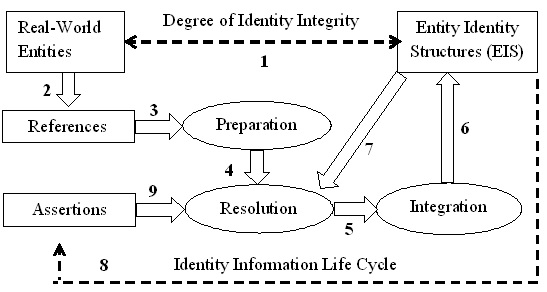
\includegraphics[width=14cm,height=7cm]{Figures/OriginalEIIM.jpg}
%\end{figure} 
%
%In this section we explain the current EIIM process that lays the foundation and acts as a background of the presented research.
%The idea of Entity Identity Information Management (EIIM) as defined by [15] is the collection and management of identity information of real-world entities with the goal of sustaining entity identity integrity. Their model of EIIM was motivated by the problem of entity resolution in information systems, particularly in the domain of MDM (Master Data Management). They define entity resolution as the process of determining whether two references to real-world objects in an information system are referring to the same object, or to different object [16]. The EIIM life cycle as proposed by them is an iterative process that combines entity resolution and data structures representing entity identity into specific operational configurations (EIIM configurations, as shown in Figure 3), that when executed in concert, work to maintain the entity identity integrity of master data over time. The EIIM framework is implemented by developing open source software known as OYSTER .

